\documentclass[a4paper, 12pt]{scrartcl}
\usepackage[utf8]{inputenc}
\usepackage{ngerman}
\usepackage{setspace}
\usepackage{geometry}
\usepackage[hidelinks]{hyperref}
\usepackage{xcolor,soul}
\usepackage{graphicx}

\geometry{a4paper, top=25mm, left=25mm, right=25mm, bottom=25mm}

\usepackage{xcolor}
\usepackage[normalem]{ulem}
\useunder{\uline}{\ulined}{}%
\DeclareUrlCommand{\bulurl}{\def\UrlFont{\ttfamily\color{blue}\ulined}}

\title{Seminar IT-Sicherheit}
\author{Kevin Seidel \\ Studiengang Informatik \\ Matrikelnummer: 943147}

\begin{document}
\pagenumbering{arabic}
\setcounter{page}{1}

Im folgenden Bericht werden die Ergebnisse von zwei verschiedenen Netzwerksimulationen dargelegt. Diese wurden nach der Vorgabe aus der {\color{blue}\uline{ \href{http://sys.cs.uos.de/lehre/rene/2013/aufgaben/PA_Blatt02.pdf}{Praktischen Aufgabe 2}}} durchgeführt. Dort wurden die zu verwendeten Durchsatzraten und die Netzwerktopologie festgelegt.
Dabei wereden zwei Szenarien betrachtet. In einem wird ein voll funktionsfähiges Netzwerk betrachtet, wohingegen im zweitem Szenario ein Netzwerk mit fehlerhafter Kabelverbindung betrachtet.
Das weitere Vorgehen dieses Berichtes orientiert sich am {\color{blue}\uline{ \href{http://sys.cs.uos.de/lehre/rene/2013/folien/Kap3-Messungen.pdf}{ Mesurement Cookbook}}}, welches in der Veranstaltung Rechnernetze vorgestellt wurde.

\section{Aufgabenstellung}
Die Aufgabe bestand darin, zwei Netzwerksimulationen mit dem Simulationsprogramm ns-3 durchzuführen. Bei diesen Simulationen ging es um die Beobachtung der Datenraten bei einer TCP-Verbindung zwischen einem Server mit 5 Clients, welche über einen Router miteinander verbunden sind.
Die erste Simulation betrachtet ein funktionierendes Netzwerk ohne Fehler, wohingegen in der zweiten Simulation eine theoretische Beschädigung der Verbindung zwischen Router und Server simuliert wird. Diese Beschädigung bewirkt einen Paketverlust von 10% auf dieser Verbindung.
Dabei soll ein Vergleich zwischen den Datenraten der beiden Simulationen erstellt werden und die Ergebnisse analysiert werden.

\section{Netzwerkmodell}
\begin{figure}[htbp]
	\centering
    \includegraphics[width=10cm]{net-topology.pdf}
  \caption{Netzwerktopologie}
  \label{Labelname}
\end{figure}
Das zu simulierende Netzwerk besteht aus fünf Clients, einem Router und einem Server. 
Der Server hat eine Verbindung zum Router. Diese erlaubt einen maximalen Durchsatz von 1Mbit/s und hat eine Verzögerung von 20 ms.
Die fünf Clients verfügen ebenfalls über jeweils eine Verbindung zum Router, welche auch über einen Durchsatz von 1Mbit/s und eine Verzögerung von 20ms verfügen.
Alle Netzwerkgeräte verfügen über eine Drop Tail Queue, das heißt es werden erst Pakete verworfen, wenn die jeweilige Queue komplett gefüllt ist.
In der Simulation wird ein TCP-Stream vom Server zu jedem Client aufgebaut, welcher über den Router führt. Jeder Client versucht dabei einen Durchsatz von 1Mbit/s zu erreichen, wobei zwischen Router und Server maximal ein Durchsatz von 1Mbit/s realisiert werden kann, welcher sich auf die Clients aufteilt.


\section{Leistungsmetrik}
Für unsere Aufgabe betrachten wir sowohl den Durchsatz der einzelnen Clients, als auch den Gesamtdurchsatz des Servers. Des Weiteren wird der aufsummierte Durchsatz betrachtet, um die Ergebnisse besser zu vergleichen.

\section{Variable Parameter}
Der einzige variable Parameter in unserem Aufbau ist die Packetverlustrate der Server-Router-Verbindung zwischen den beiden Simulationen. In der ersten Simulation beträgt diese 0\%, heißt also, dass alle Pakete ordnungsgemäß übertragen werden. In der zweiten Simulation gehen 10\% der Pakete  zwischen Router und Server verloren.

\section{Modellüberführung in Software}
Für die Simulation wird die Software ns-3 verwendet. Dabei handelt es sich um einen Simulator für Netzwerkverbindungen. 
Zu Beginn der Simulation werden noch keine Daten gesendet. Nach 5 Sekunden startet der Server damit, Packete an den Client0 zu senden. Darauffolgend starten die anderen TCP-Streams in 5 Sekunden Abständen. Nach 25 Sekunden sind nun Streams zu allen 5 Clients aktiv. Diese werden für 40 weitere Sekunden aufrecht erhalten, bis sie bei Sekunde 65 beendet werden. Nach insgesamt 70 Sekunden endet die Simulation.

Die Größe der TCP-Packete die vom Server zu den Clients gesendet werden, beträgt 578 Byte. Die  Acknowledgements und Synchronize-Acknowledgement haben eine Größe von 42 Byte.

\section{Konfiguration zur Datenerzeugung}
Das Simulationsprogramm erzeugt für die spätere Analyse ein ASCII-Trace mit allen Packeten. Zusätzlich wird eine XML-Datei erzeugt, welche es mittels des Programmes NetAnim erlaubt, die gesendeten Packete grafisch in einer animierten Form darzustellen. Diese Dateien wurden nach dem auf dem Aufgabenblatt geforderten Namensschema erstellt. \\

Erste Simulation: \\
ASCII-Trace: ReNe\_SoSe\_2013\_PA2a\_943147.tr \\
NetAnim : ReNe\_SoSe\_2013\_PA2a\_943147.xml  \\
Zweite Simulation: \\
ASCII-Trace: ReNe\_SoSe\_2013\_PA2b\_943147.tr \\
NetAnim : ReNe\_SoSe\_2013\_PA2b\_943147.xml  \\

\section{Simulationsdurchführung und Datenerfassung}
Die beiden Simulationen wurden mit den bereits oben gegebenen Parametern durchgeführt. Für die weiteren Untersuchungen wurde der dadurch erstellte ASCII-Trace verwendet.
Zur späteren Weiterverarbeitung wurden aus dem ASCII-Trace die relevanten Daten extrahiert und in verschiedene CSV-Files geschrieben. Dabei wird ein CSV-File mit dem Durchsatz pro Zeiteinheit mit aufsummiertem Durchsatz, eines für den Durchsatz pro Zeiteinheit ohne aufsummierten Durchsatz und eines für den gesamten Datendurchsatz erstellt. Die geschieht mit Hilfe eines selbstgeschriebenem Python-Programmes. 

\section{Präsentation und Interpretation der Ergebnisse}
Für die grafische Präsentation der Ergebnisse wird die Programmiersprache R genutzt, welche sich gut für die Erstellung von Plots und Diagrammen eignet. 
Für die grafische Darstellung wurde in den CSV-Files ein Intervall von 0.25 Sekunden benutzt.

Bei der ersten Simulation ergab sich eine fast vollständige Auslastung der Verbindung zwischen Server und Router, wie auch im nachfolgenden Diagramm zu sehen.

\begin{figure}[htbp]
	\centering
    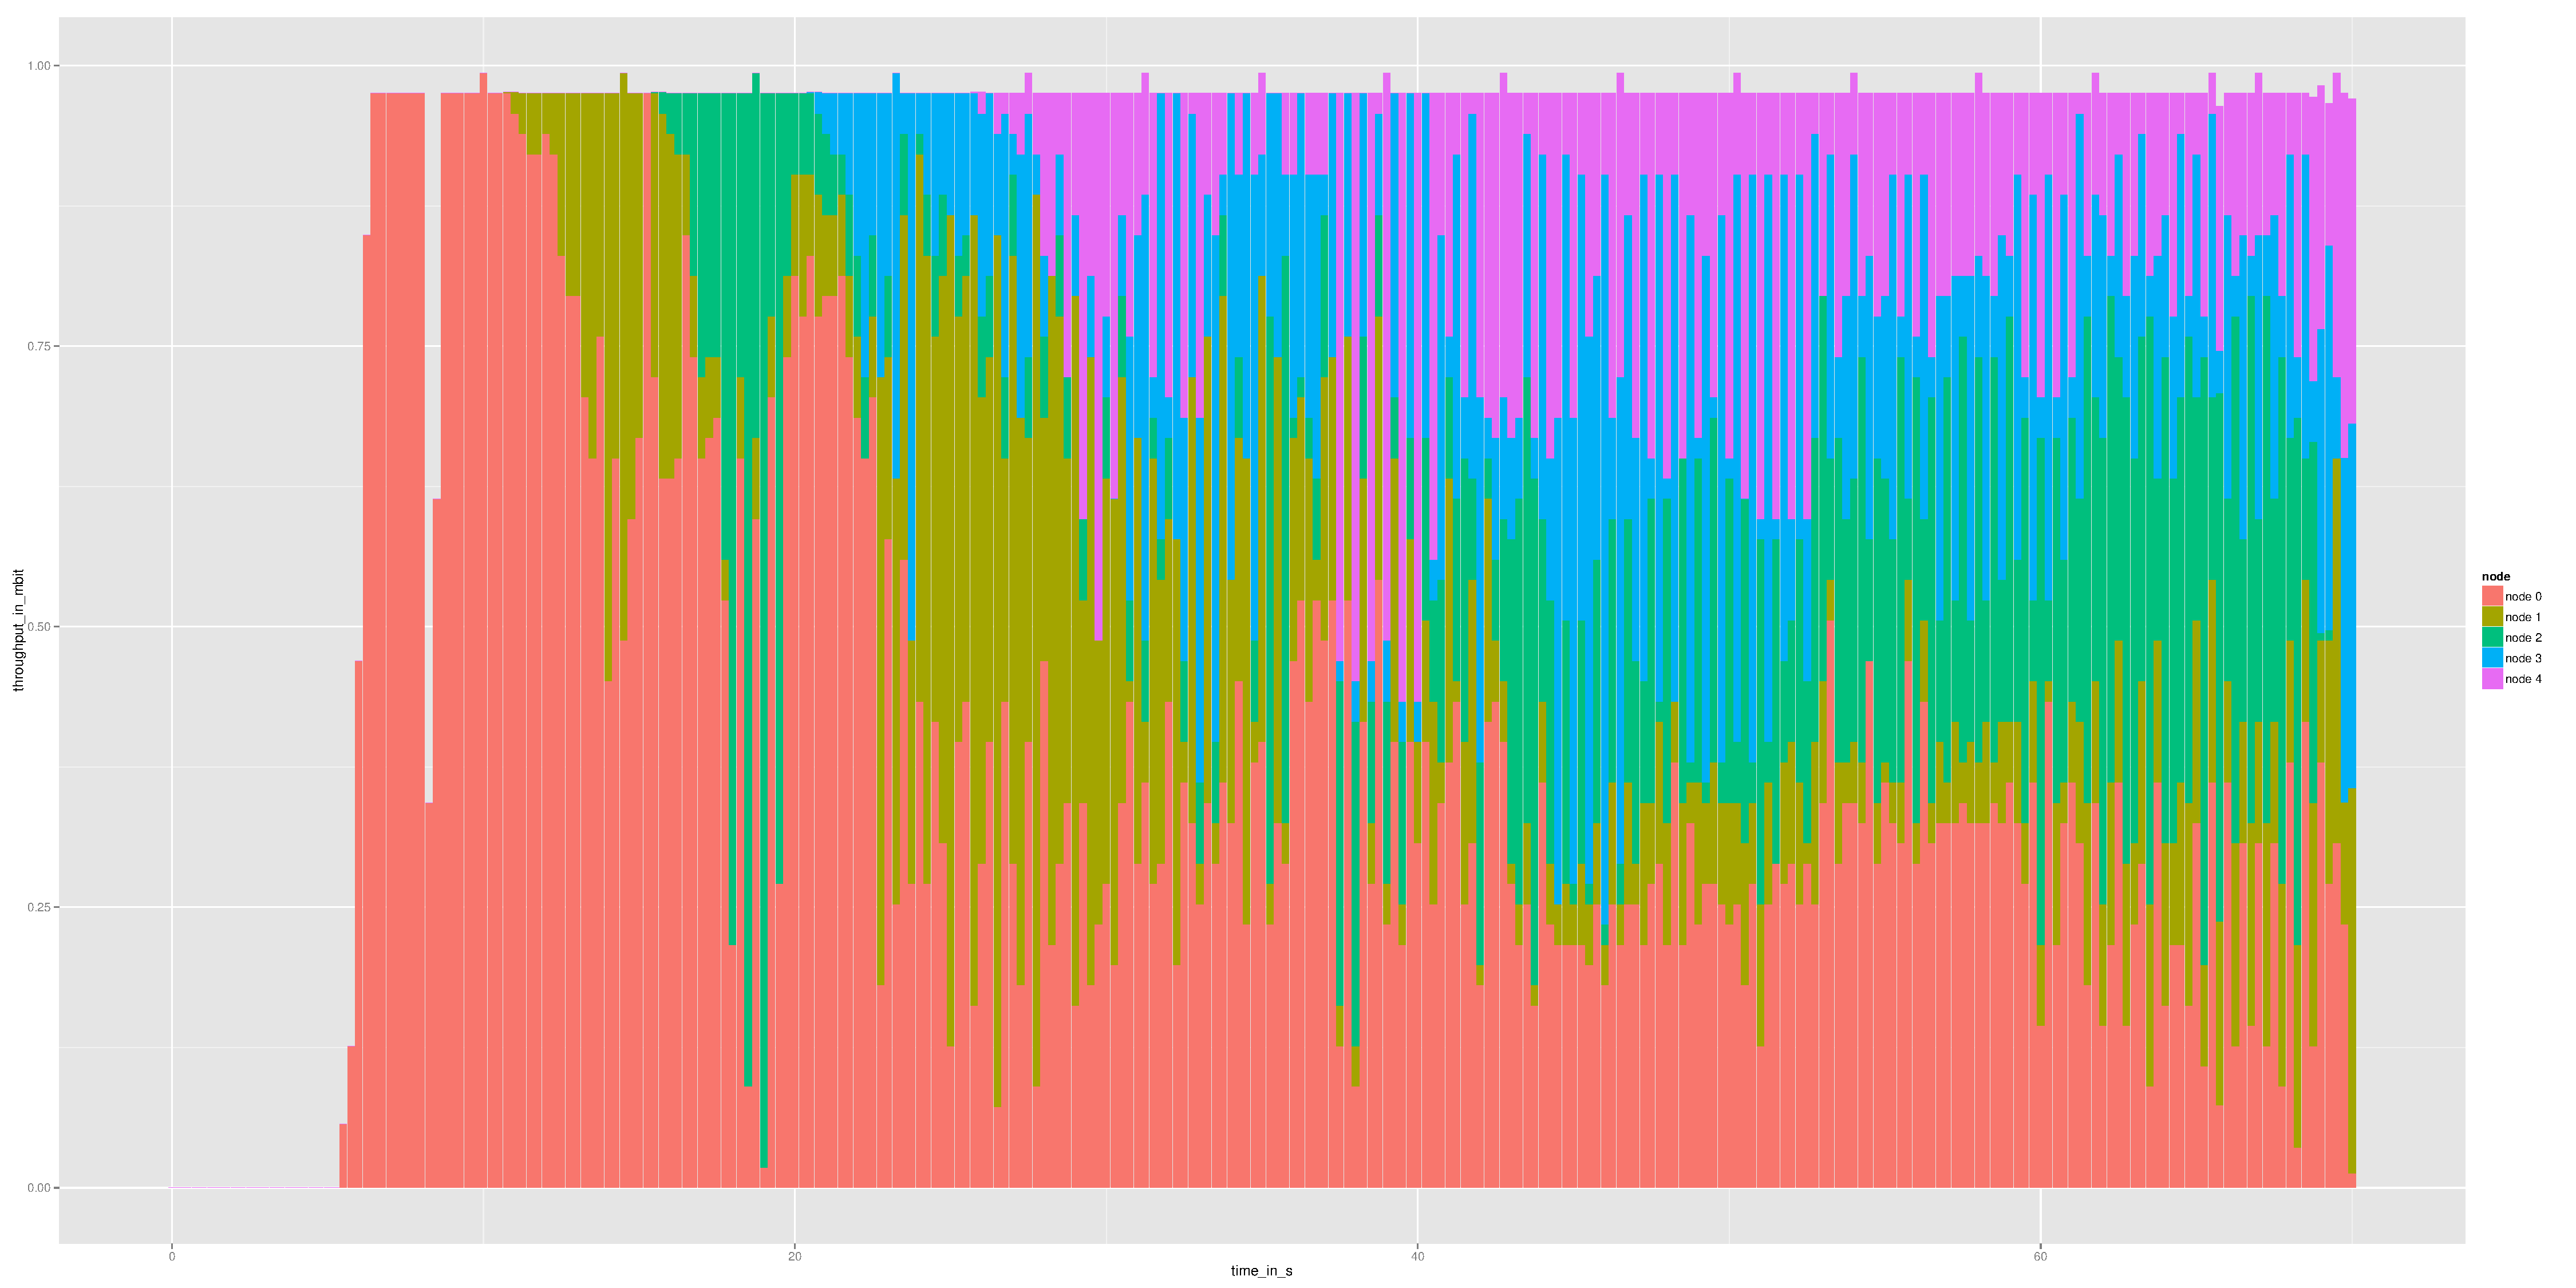
\includegraphics[width=15cm]{ReNe_SoSe_2013_PA2a_943147_stackedbar.pdf}
  \caption{Durchsatz der einzelnen Clients}
  \label{Labelname}
\end{figure}

Da die Verbindung zwischen Server und Router der Flaschenhals des Aufbaus ist, ist nur ein maximaler Durchsatz von 1Mbps möglich, welcher unter den einzelnen Clients verteilt wird. Im Diagram ist gut zu erkennen, dass die einzelnen Datenraten der Clients relativ stark schwanken, der Gesamtdurchsatz jedoch ziemlich konsant bleibt.



Bei der zweiten Simulation zeigt sich ein komplett anderes Bild. 

\begin{figure}[htbp]
	\centering
    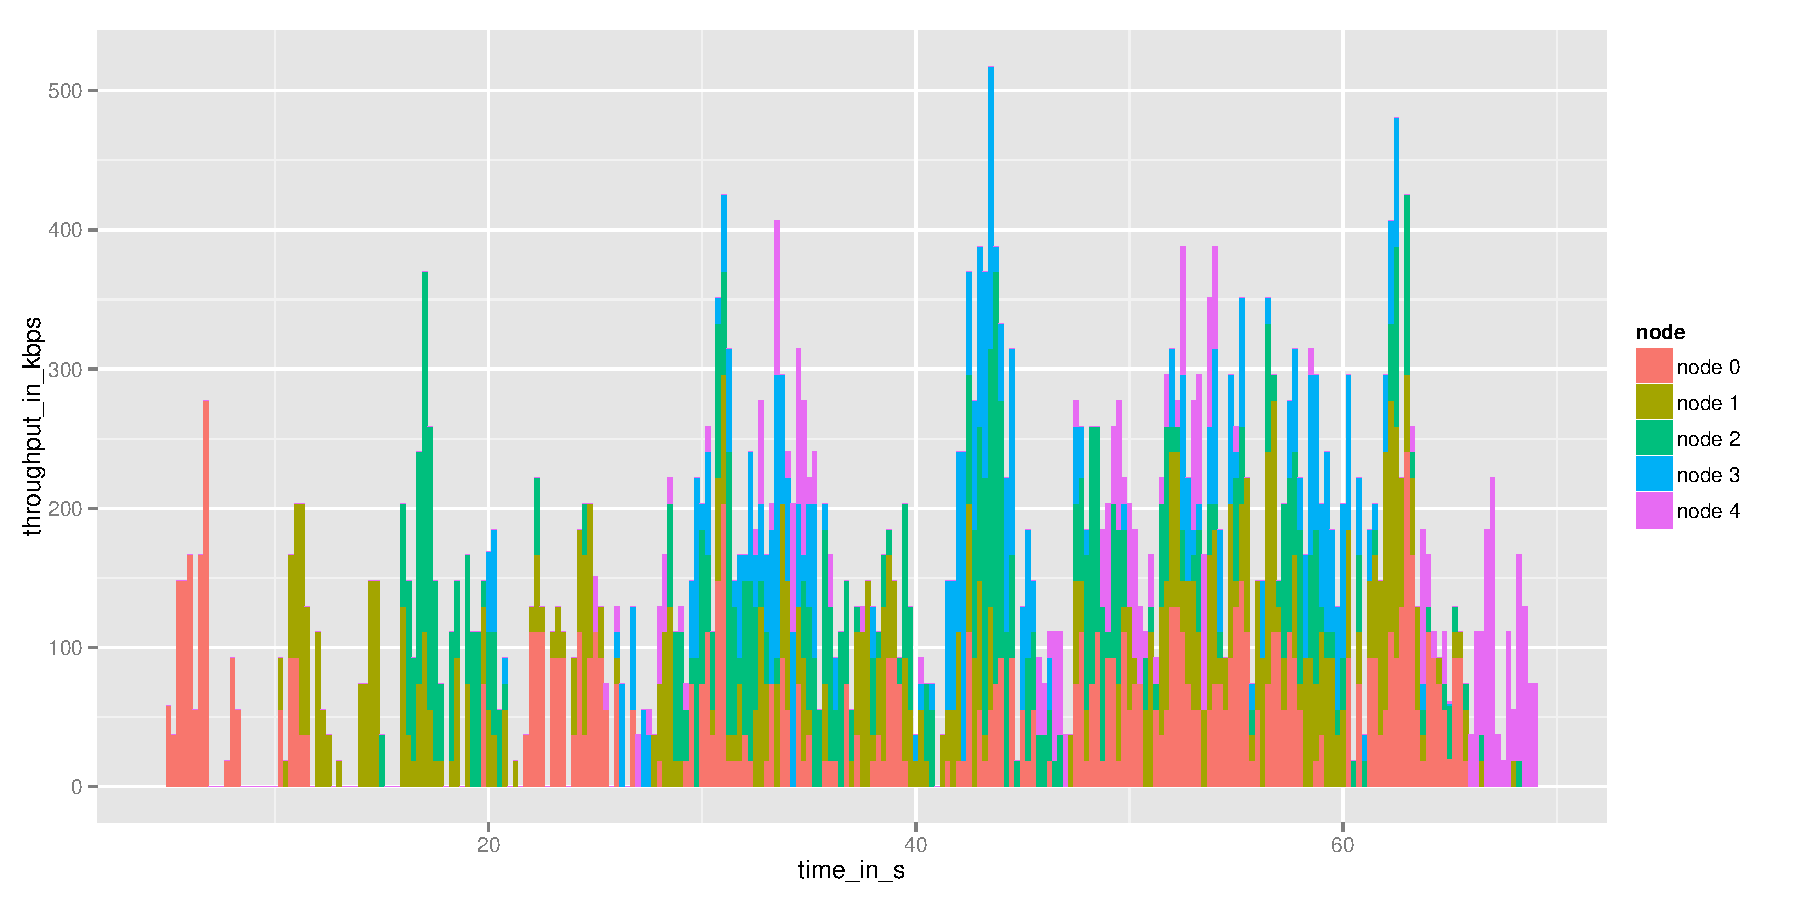
\includegraphics[width=15cm]{ReNe_SoSe_2013_PA2b_943147_stackedbar.pdf}
  \caption{Durchsatz der einzelnen Clients}
  \label{Labelname}
\end{figure}

Hier schwankt nicht nur der Durchsatz der einzelnen Clients, sondern auch der Gesamtdurchsatz stark.
Außerdem hat sich der maximale Durchsatz halbiert und dass obwohl nur 10\% der Packete verloren geht. Dies lässt sich auf die Funktionsweise von TCP zurückführen, welches versucht sicherzustellen, dass alle gesendeten Packet ankommen. Dazu wird für jedes Packet ein Acknowledgement gesendet, um den Empfang quasi zu Quittieren. Geht nun ein Packet oder das dazugehörige Achnowledgement verloren

\end{document}